\begin{figure}[!h]
\centering
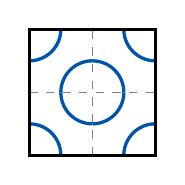
\begin{tikzpicture}[scale=0.8]
  \foreach \a/\b/\theta in {
    0/0/0, 1/1/180,
    1/1/270, 2/0/90,
    0/2/270, 1/1/90,
    1/1/0, 2/2/180} {
    \draw[very thick, draw={rgb:red,0;green,1;blue,2}, domain=\theta:\theta+90] plot ({0.5*cos(\x) + \a}, {0.5*sin(\x) + \b});
  }
  \draw[gray, dashed] (0,0) grid (2,2);
  \draw[very thick] (0,0) rectangle (2,2);
\end{tikzpicture}
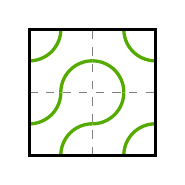
\begin{tikzpicture}[scale=0.8]
  \draw[gray, dashed] (0,0) grid (2,2);
  \foreach \a/\b/\theta in {
    0/1/270, 1/0/90,
    1/1/270, 2/0/90,
    0/2/270, 1/1/90,
    1/1/0, 2/2/180} {
    \draw[very thick, draw={rgb:red,1;green,2;blue,0}, domain=\theta:\theta+90] plot ({0.5*cos(\x) + \a}, {0.5*sin(\x) + \b});
  }
  \draw[very thick] (0,0) rectangle (2,2);
\end{tikzpicture}
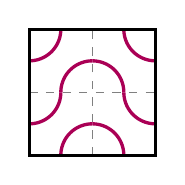
\begin{tikzpicture}[scale=0.8]
  \draw[gray, dashed] (0,0) grid (2,2);
  \foreach \a/\b/\theta in {
    0/1/270, 1/0/90,
    1/0/0, 2/1/180,
    0/2/270, 1/1/90,
    1/1/0, 2/2/180} {
    \draw[very thick, draw={rgb:red,2;green,0;blue,1}, domain=\theta:\theta+90] plot ({0.5*cos(\x) + \a}, {0.5*sin(\x) + \b});
  }
  \draw[very thick] (0,0) rectangle (2,2);
\end{tikzpicture}
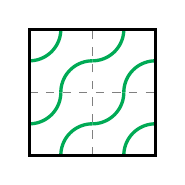
\begin{tikzpicture}[scale=0.8]
  \draw[gray, dashed] (0,0) grid (2,2);
  \foreach \a/\b/\theta in {
    0/1/270, 1/0/90,
    1/1/270, 2/0/90,
    0/2/270, 1/1/90,
    1/2/270, 2/1/90} {
    \draw[very thick, draw={rgb:red,0;green,2;blue,1}, domain=\theta:\theta+90] plot ({0.5*cos(\x) + \a}, {0.5*sin(\x) + \b});
  }
  \draw[very thick] (0,0) rectangle (2,2);
\end{tikzpicture}
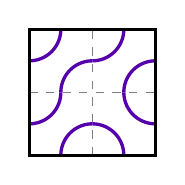
\begin{tikzpicture}[scale=0.8]
  \draw[gray, dashed] (0,0) grid (2,2);
  \foreach \a/\b/\theta in {
    0/1/270, 1/0/90,
    1/0/0, 2/1/180,
    0/2/270, 1/1/90,
    1/2/270, 2/1/90} {
    \draw[very thick, draw={rgb:red,1;green,0;blue,2}, domain=\theta:\theta+90] plot ({0.5*cos(\x) + \a}, {0.5*sin(\x) + \b});
  }
  \draw[very thick] (0,0) rectangle (2,2);
\end{tikzpicture}
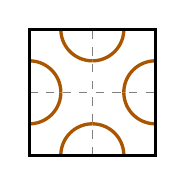
\begin{tikzpicture}[scale=0.8]
  \draw[gray, dashed] (0,0) grid (2,2);
  \foreach \a/\b/\theta in {
    0/1/270, 1/0/90,
    1/0/0, 2/1/180,
    0/1/0, 1/2/180,
    1/2/270, 2/1/90} {
    \draw[very thick, draw={rgb:red,2;green,1;blue,0}, domain=\theta:\theta+90] plot ({0.5*cos(\x) + \a}, {0.5*sin(\x) + \b});
  }
  \draw[very thick] (0,0) rectangle (2,2);
\end{tikzpicture}
\\ \vspace{2pt}
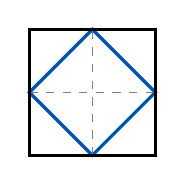
\begin{tikzpicture}[scale=0.8]
  \draw[very thick, draw={rgb:red,0;green,1;blue,2}]
    (0,1)--(1,0)--(2,1)--(1,2)--cycle;
  \draw[gray, dashed] (0,0) grid (2,2);
  \draw[very thick] (0,0) rectangle (2,2);
\end{tikzpicture}
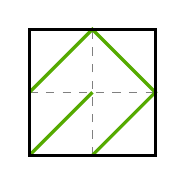
\begin{tikzpicture}[scale=0.8]
  \draw[gray, dashed] (0,0) grid (2,2);
  \draw[very thick, draw={rgb:red,1;green,2;blue,0}]
    (0,0)--(1,1)
    (0,1)--(1,2)--(2,1)--(1,0);
  \draw[very thick] (0,0) rectangle (2,2);
\end{tikzpicture}
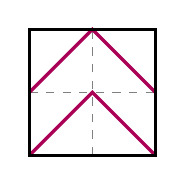
\begin{tikzpicture}[scale=0.8]
  \draw[gray, dashed] (0,0) grid (2,2);
  \draw[very thick, draw={rgb:red,2;green,0;blue,1}]
    (0,0)--(1,1)--(2,0)
    (0,1)--(1,2)--(2,1);
  \draw[very thick] (0,0) rectangle (2,2);
\end{tikzpicture}
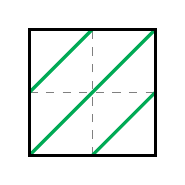
\begin{tikzpicture}[scale=0.8]
  \draw[gray, dashed] (0,0) grid (2,2);
  \draw[very thick, draw={rgb:red,0;green,2;blue,1}]
    (0,1)--(1,2)
    (0,0)--(2,2)
    (1,0)--(2,1);
  \draw[very thick] (0,0) rectangle (2,2);
\end{tikzpicture}
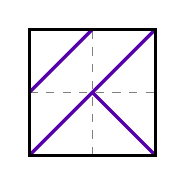
\begin{tikzpicture}[scale=0.8]
  \draw[gray, dashed] (0,0) grid (2,2);
  \draw[very thick, draw={rgb:red,1;green,0;blue,2}]
    (0,1)--(1,2)
    (0,0)--(2,2)
    (1,1)--(2,0);
  \draw[very thick] (0,0) rectangle (2,2);
\end{tikzpicture}
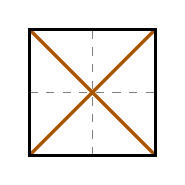
\begin{tikzpicture}[scale=0.8]
  \draw[gray, dashed] (0,0) grid (2,2);
  \draw[very thick, draw={rgb:red,2;green,1;blue,0}]
    (2,0)--(0,2)
    (0,0)--(2,2);
  \draw[very thick] (0,0) rectangle (2,2);
\end{tikzpicture}
\caption {
  An example of the $a(2) = 6$ different ways to fill the $2 \times 2$ grid
  with diagonal tiles up to dihedral action of the square.
}
\end{figure}